\documentclass[border=3pt]{standalone}
% Preâmbulo compartilhado pelos diagramas TikZ da aula 8 de IHR (Métodos de Pesquisa)
\usepackage[T1]{fontenc}
\usepackage[utf8]{inputenc}
\usepackage{lmodern}
\usepackage{amsmath}
\usepackage{xcolor}
\usepackage{tikz}
\usetikzlibrary{arrows.meta,angles,quotes,decorations.pathmorphing,decorations.pathreplacing,calc,
                positioning,shapes.geometric,shapes.misc,backgrounds,fit,
                math}

% Paleta (mesma dos SVGs originais)
% Paleta da disciplina de IHR: acento azul (#1A6FB5), cor de destaque do tema.
% (o nome "dblue" é mantido para não alterar todos os diagramas)
\definecolor{dblue}{HTML}{1A6FB5}
\definecolor{dorange}{HTML}{B3541E}
\definecolor{dgreen}{HTML}{4A7C59}
\definecolor{dred}{HTML}{9C4B4B}
\definecolor{dcream}{HTML}{F4F1EA}
\definecolor{dshade}{HTML}{DDD7C9}

% Função gaussiana (não normalizada por padrão de escala visual)
\pgfmathdeclarefunction{gauss}{3}{%
  \pgfmathparse{1/(#3*sqrt(2*pi))*exp(-((#1-#2)^2)/(2*#3^2))}%
}

% Estilos comuns (prefixo d... para não colidir com chaves internas do pgf)
\tikzset{
  >={Stealth[length=2mm]},
  dguide/.style={gray!55, dashed, line width=0.4pt},
  daxis/.style={gray!60, line width=0.7pt, ->},
  dbody/.style={fill=black!3, draw=black!80, line width=1pt},
  dacc/.style={draw=dblue, line width=1pt},
  dlbl/.style={black!55, font=\small},
  dsub/.style={black!45, font=\footnotesize},
  dstate/.style={circle, draw=black!80, fill=dcream, line width=1pt,
                 minimum size=17mm, font=\large, inner sep=1pt},
  dobs/.style={circle, draw=black!80, fill=dshade, line width=1pt,
               minimum size=14mm, font=\large, inner sep=1pt},
  dbox/.style={rounded corners=2pt, draw=black!80, fill=dcream, line width=1pt,
               align=center, inner sep=6pt},
  dop/.style={circle, draw=black!80, fill=white, line width=1pt,
              minimum size=6mm, inner sep=0pt, font=\small},
  dtrans/.style={->, dblue, line width=1pt},
  dmeas/.style={->, dorange, line width=1pt},
  dcurve/.style={line width=1pt, dblue},
  dcurveb/.style={line width=1.4pt, dorange},
}

\begin{document}
\hyphenpenalty=10000 \exhyphenpenalty=10000 \tolerance=9999 \emergencystretch=3em
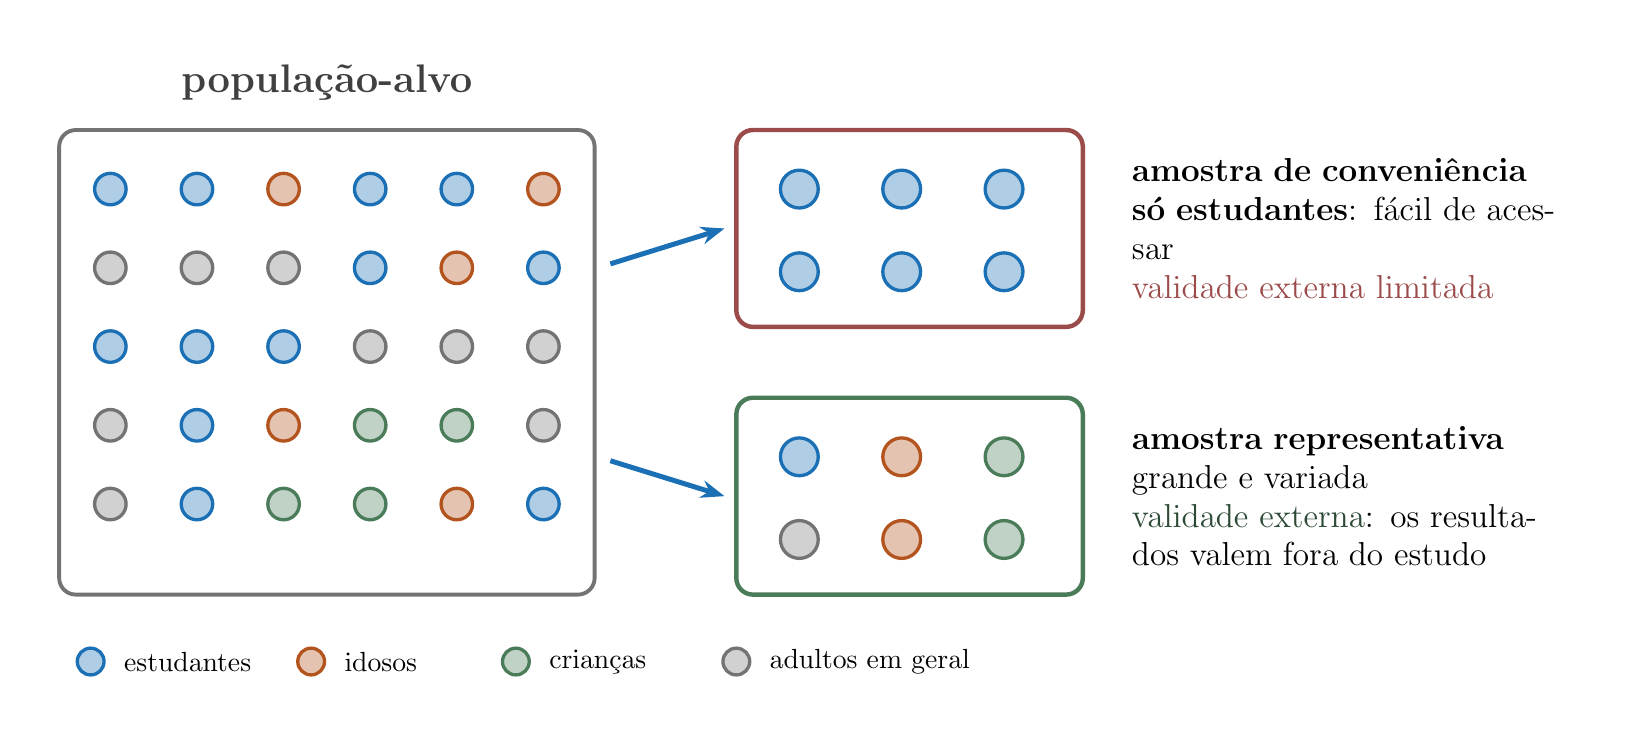
\begin{tikzpicture}[x=1cm,y=1cm]
  \useasboundingbox (-0.4,0.7) rectangle (19.6,9.4);
  \node[font=\Large\bfseries, black!75] at (3.4,8.7) {população-alvo};
  \draw[black!55, line width=1.4pt, rounded corners=6pt] (0,2.2) rectangle (6.8,8.1);
  \draw[dblue, fill=dblue!35, line width=1.2pt] (0.65,7.35) circle (0.20);
  \draw[dblue, fill=dblue!35, line width=1.2pt] (1.75,7.35) circle (0.20);
  \draw[dorange, fill=dorange!35, line width=1.2pt] (2.85,7.35) circle (0.20);
  \draw[dblue, fill=dblue!35, line width=1.2pt] (3.95,7.35) circle (0.20);
  \draw[dblue, fill=dblue!35, line width=1.2pt] (5.05,7.35) circle (0.20);
  \draw[dorange, fill=dorange!35, line width=1.2pt] (6.15,7.35) circle (0.20);
  \draw[black!55, fill=black!18, line width=1.2pt] (0.65,6.35) circle (0.20);
  \draw[black!55, fill=black!18, line width=1.2pt] (1.75,6.35) circle (0.20);
  \draw[black!55, fill=black!18, line width=1.2pt] (2.85,6.35) circle (0.20);
  \draw[dblue, fill=dblue!35, line width=1.2pt] (3.95,6.35) circle (0.20);
  \draw[dorange, fill=dorange!35, line width=1.2pt] (5.05,6.35) circle (0.20);
  \draw[dblue, fill=dblue!35, line width=1.2pt] (6.15,6.35) circle (0.20);
  \draw[dblue, fill=dblue!35, line width=1.2pt] (0.65,5.35) circle (0.20);
  \draw[dblue, fill=dblue!35, line width=1.2pt] (1.75,5.35) circle (0.20);
  \draw[dblue, fill=dblue!35, line width=1.2pt] (2.85,5.35) circle (0.20);
  \draw[black!55, fill=black!18, line width=1.2pt] (3.95,5.35) circle (0.20);
  \draw[black!55, fill=black!18, line width=1.2pt] (5.05,5.35) circle (0.20);
  \draw[black!55, fill=black!18, line width=1.2pt] (6.15,5.35) circle (0.20);
  \draw[black!55, fill=black!18, line width=1.2pt] (0.65,4.35) circle (0.20);
  \draw[dblue, fill=dblue!35, line width=1.2pt] (1.75,4.35) circle (0.20);
  \draw[dorange, fill=dorange!35, line width=1.2pt] (2.85,4.35) circle (0.20);
  \draw[dgreen, fill=dgreen!35, line width=1.2pt] (3.95,4.35) circle (0.20);
  \draw[dgreen, fill=dgreen!35, line width=1.2pt] (5.05,4.35) circle (0.20);
  \draw[black!55, fill=black!18, line width=1.2pt] (6.15,4.35) circle (0.20);
  \draw[black!55, fill=black!18, line width=1.2pt] (0.65,3.35) circle (0.20);
  \draw[dblue, fill=dblue!35, line width=1.2pt] (1.75,3.35) circle (0.20);
  \draw[dgreen, fill=dgreen!35, line width=1.2pt] (2.85,3.35) circle (0.20);
  \draw[dgreen, fill=dgreen!35, line width=1.2pt] (3.95,3.35) circle (0.20);
  \draw[dorange, fill=dorange!35, line width=1.2pt] (5.05,3.35) circle (0.20);
  \draw[dblue, fill=dblue!35, line width=1.2pt] (6.15,3.35) circle (0.20);
  \draw[dred, line width=1.6pt, rounded corners=6pt] (8.6,5.6) rectangle (13.0,8.1);
  \draw[dblue, fill=dblue!35, line width=1.2pt] (9.40,7.35) circle (0.24);
  \draw[dblue, fill=dblue!35, line width=1.2pt] (10.70,7.35) circle (0.24);
  \draw[dblue, fill=dblue!35, line width=1.2pt] (12.00,7.35) circle (0.24);
  \draw[dblue, fill=dblue!35, line width=1.2pt] (9.40,6.30) circle (0.24);
  \draw[dblue, fill=dblue!35, line width=1.2pt] (10.70,6.30) circle (0.24);
  \draw[dblue, fill=dblue!35, line width=1.2pt] (12.00,6.30) circle (0.24);
  \node[font=\large, text width=5.6cm, align=left, anchor=west] at (13.5,6.85) {\textbf{amostra de conveniência}\\ \textbf{só estudantes}: fácil de acessar\\ \textcolor{dred}{validade externa limitada}};
  \draw[dgreen, line width=1.6pt, rounded corners=6pt] (8.6,2.2) rectangle (13.0,4.7);
  \draw[dblue, fill=dblue!35, line width=1.2pt] (9.40,3.95) circle (0.24);
  \draw[dorange, fill=dorange!35, line width=1.2pt] (10.70,3.95) circle (0.24);
  \draw[dgreen, fill=dgreen!35, line width=1.2pt] (12.00,3.95) circle (0.24);
  \draw[black!55, fill=black!18, line width=1.2pt] (9.40,2.90) circle (0.24);
  \draw[dorange, fill=dorange!35, line width=1.2pt] (10.70,2.90) circle (0.24);
  \draw[dgreen, fill=dgreen!35, line width=1.2pt] (12.00,2.90) circle (0.24);
  \node[font=\large, text width=5.6cm, align=left, anchor=west] at (13.5,3.45) {\textbf{amostra representativa}\\ grande e variada\\ \textcolor{dgreen!60!black}{validade externa}: os resultados valem fora do estudo};
  \draw[dtrans, line width=1.8pt, -{Stealth[length=3mm]}] (7.0,6.4) -- (8.45,6.85);
  \draw[dtrans, line width=1.8pt, -{Stealth[length=3mm]}] (7.0,3.9) -- (8.45,3.45);
  \draw[dblue, fill=dblue!35, line width=1.2pt] (0.40,1.35) circle (0.17);
  \node[font=\normalsize, anchor=west] at (0.70,1.35) {estudantes};
  \draw[dorange, fill=dorange!35, line width=1.2pt] (3.20,1.35) circle (0.17);
  \node[font=\normalsize, anchor=west] at (3.50,1.35) {idosos};
  \draw[dgreen, fill=dgreen!35, line width=1.2pt] (5.80,1.35) circle (0.17);
  \node[font=\normalsize, anchor=west] at (6.10,1.35) {crianças};
  \draw[black!55, fill=black!18, line width=1.2pt] (8.60,1.35) circle (0.17);
  \node[font=\normalsize, anchor=west] at (8.90,1.35) {adultos em geral};
\end{tikzpicture}
\end{document}
